\chapter{Construcción del sistema}
\label{cap:Construccion}

Este capítulo detalla la fase de construcción de la aplicación, comenzando con la toma de requistos, la toma de desiciones de diseño en todo ámbito y culmina con como se realizó la implementación.

\section{Toma de requisitos}
\label{sec:Requisitos}

Se han construido dos aplicaciones; La primera es el visualizador, el que se encarga de aplicar los filtros y mostrar la información correspondiente a los puntos donde se han detectado necesidades y la segunda corresponde a aquella que realiza la recepción del flujo de datos desde \textit{Twitter} y su paso por el clasificador. Las razones por las que se consideraron dos aplicaciones separadas se especificarán en la sección \ref{sec:Diseno}.\\

Esta sección detallará los requisitos de las aplicaciones, descritos como historias de usuario. Éstos señalan las necesidades de los clientes - Profesores guía y co-guía - expresadas en sucesivas reuniones mantenidas en el Departamento de Ingeniería Informática de la universidad donde se mostró, semana a semana, avances en la aplicación y se señalaron los cambios que habían de hacerse o que serían deseables.\\

Estos requisitos tendrán la siguiente nomenclatura para su identificación: Aquellos que guarden relación con la aplicación de detección se identificarán como 'HU-cXX' donde XX corresponderá al número del requisito; 'HU-vYY' para aquellas que correspondan a la aplicación interfáz donde, al igual que en el caso anterior, YY corresponderá al número del requisito.\\

La tabla \ref{tab:ReqTotales} presenta la totalidad de requisitos, tanto de la aplicación visualizador como del detector de necesitades.\\

\begin{table}[H]
\centering
\caption{Historias de usuario}
\label{tab:ReqTotales}
\begin{tabular}{cl}
\hline
\textbf{Identificador}       & \multicolumn{1}{c}{\textbf{Historia de usuario}}                                                                                                                                                                                                                                                                                                                                      \\ \hline
\multicolumn{1}{|c|}{HU-c00} & \multicolumn{1}{l|}{\begin{tabular}[c]{@{}l@{}}Como cliente quiero capturar necesidades de la población en tiempo real \\ cuando el país se encuentre en un escenario de catástrofe natural para poder \\ contar con información para asistir a la población afectada.\end{tabular}}                                                                                                  \\ \hline
\multicolumn{1}{|c|}{HU-c01} & \multicolumn{1}{l|}{\begin{tabular}[c]{@{}l@{}}Como cliente quiero que las necesidades detectadas se recojan desde la \\ información generadas en redes sociales redes sociales para que las personas\\ sean la fuente primaria.\end{tabular}}                                                                                                                                        \\ \hline
\multicolumn{1}{|c|}{HU-c02} & \multicolumn{1}{l|}{\begin{tabular}[c]{@{}l@{}}Como cliente quiero que la búsqueda de necesidades se vea enriquecida para\\  abarcar nuevos términos de búsqueda para abarcar un conjunto mayor de \\ información.\end{tabular}}                                                                                                                                                      \\ \hline
\multicolumn{1}{|c|}{HU-v00} & \multicolumn{1}{l|}{\begin{tabular}[c]{@{}l@{}}Como usuario quiero una interfaz donde pueda visualizar el comportamiento \\ del sistema de detección para poder interactuar con el.\end{tabular}}                                                                                                                                                                                     \\ \hline
\multicolumn{1}{|c|}{HU-v01} & \multicolumn{1}{l|}{\begin{tabular}[c]{@{}l@{}}Como cliente quiero que las necesidades detectadas puedan ser asociadas a \\ un punto en un mapa geográfico para poder identificar el lugar físico de su \\ fuente.\end{tabular}}                                                                                                                                                      \\ \hline
\multicolumn{1}{|c|}{HU-v02} & \multicolumn{1}{l|}{\begin{tabular}[c]{@{}l@{}}Como usuario quiero que puedan aplicarse filtros a la visualización de los \\ puntos de modo que según la distancia entre ellos, cuáles se quieran mostrar\\ y el nivel de acercamiento que tenga el mapa se entreguen diferentes formas\\ de mostrar la información para que la información se visualice con facilidad.\end{tabular}} \\ \hline
\multicolumn{1}{|c|}{HU-v03} & \multicolumn{1}{l|}{\begin{tabular}[c]{@{}l@{}}Como usuario quiero que la visualización de eventos se realice en tiempo \\ real para tomar decisiones rápidas cuando la situación lo amerite.\end{tabular}}                                                                                                                                                                           \\ \hline
\multicolumn{1}{|c|}{HU-v04} & \multicolumn{1}{l|}{\begin{tabular}[c]{@{}l@{}}Como usuario quiero visualizar eventos pasados, además quiero poder \\ seleccionar un intervalo de tiempo y que el sistema muestre todos los \\ eventos que se hayan detectado dentro de aquel intervalo de modo que \\ pueda realizarse una análisis a posteriori de la emergencia.\end{tabular}}                                     \\ \hline
\multicolumn{1}{|c|}{HU-v05} & \multicolumn{1}{l|}{\begin{tabular}[c]{@{}l@{}}Como usuario quiero poder especificar términos de búsqueda para acotar la\\  búsqueda a aquel contenido que contenga elementos que se correspondan \\ con ellos.\end{tabular}}                                                                                                                                                         \\ \hline
\multicolumn{1}{|c|}{HU-v06} & \multicolumn{1}{l|}{\begin{tabular}[c]{@{}l@{}}Como usuario quiero que cada punto, correspondiente a una necesidad \\ específica, tenga un diseño particular fácilmente identificable.\end{tabular}}                                                                                                                                                                                  \\ \hline
\multicolumn{1}{|c|}{HU-07}  & \multicolumn{1}{l|}{\begin{tabular}[c]{@{}l@{}}Como usuario quiero que sea posible visualizar estadísticas del procesamiento\\ de la aplicación por consulta.\end{tabular}}                                                                                                                                                                                                           \\ \hline
\multicolumn{1}{|c|}{HU-08}  & \multicolumn{1}{l|}{\begin{tabular}[c]{@{}l@{}}Como usuario quiero poder modificar cuánto tiempo se visualizará un evento \\ antes de que sea considerado antiguo y cada cuánto tiempo se añadirá la\\ información de los nuevos eventos.\end{tabular}}                                                                                                                               \\ \hline
\end{tabular}
\end{table}

Estas historias de usuario se corresponden con los criterios de aceptación descritos en la tabla \ref{tab:criteriosAceptacion} que se presenta a continuación.

\textbf{Faltan criterios, conversarlo con profes}

\section{Desiciones de diseño e Implementación}
\label{sec:Diseno}

El desarrollo de la aplicación, entonces, será guiado por cumplir las historias de usuario descritas en la tabla \ref{tab:ReqTotales}. Para ello se trata cada historia como un problema individual que luego han de ser constituidas en la aplicación final.\\

A continuación se presenta cómo se abordó cada historia desde el punto de vista del diseño previo a la implementación. Además al final de esta sección se entrega una visión de la arquitectura final del sistema.

\subsection{Historia de usuario HU-c00}
\label{subsec:HU-c00}

Dado el contexto del funcionamiento del sistema, éste ha de entregar respuestas rápidas ante una emergencia; para ello, y como es descrito en esta historia de usuario, se requiere de un sistema capaz de procesar eventos en tiempo real que, dado el \textit{peak} de información que recibirá el sistema deberá ser escalable. El problema en este punto es el cómo construir un sistema que cumpla capáz de identificar necesidades y que posea esta, no menor, característica.\\

En primer lugar se consideraron sistemas de procesamiento distribuido; estos sistemas tienen la particularidad de ser una red de computadores (nodos, en general), que el usuario percibe como un solo gran sistema. Estos sistemas pueden ser de diversos tamaños, y suelen ser confiables, pues si un componente (nodo) falla, otro será capaz de reemplazarlo. \cite{DefSPD}. En un inicio se consideraron tres plataformas sobre las cuales podría construirse un sistema que pudiese cumplir con lo solicitado; dichas plataformas fueron Apache S4, Apache Storm y Apache Spark.\\

Apache S4, pese a su simplicidad, no continuó con su desarrollo luego del año 2013 y nunca tuvo una versión estable 1.0, razones por las cuales se dejó como segunda opción. Apache Spark, pese a contar con continuos \textit{releases}, una comunidad de desarrolladores no menor y permitir la elaboración de sistemas escalables no era lo que se buscaba en aquel momento como herramienta de desarrollo, al momento de consultar con los, en este caso, clientes, éstos esperaban que el sistema, internamente, se comportara según el paradigma de procesamiento de \textit{streams}, por medio de operadores dispuestos en un grafo. Por ello finalmente se optó por Apache Storm; Storm permite construir sistemas que cumplan con las características de un sistema distribuido, como lo son: Escalabilidad (Tanto horizontal como vertical) y tolerancia a fallos (como la capacidad de un sistema para realizar correctamente y en todo momento aquello para lo que fue diseñado). Estos sistemas estan compuestos por dos tipos de elementos: Spout y Bolt, que fueron descritos en el capítulo \ref{cap:MarcTeorico}. Al combinar esos elementos se da origen a un grafo dirigido, como el presentado en la Figura \ref{fig:stormBeLike} en la página ~\pageref{fig:stormBeLike}, donde cada elemento de procesamiento (\textit{bolt}), cumple con una determinada tarea utilizando como entrada la salida del elemento anterior.\\

Teniendo ya en consideración lo anterior el problema se traducía en cuál debería ser el procesamiendo que ha de aplicarse a los datos de entrada para capturar las necesidades. En primer lugar habrá que definir cuál y cómo será o serán las entradas del sistema para continuar la definición de los elementos con posterioridad.\\

La definición de las entradas del sistema se especificarán en la sección \ref{subsec:HU-c01}, mientras que el detalle de los elementos necesarios para cumplir esta historia de usuario se detallarán en la sección \ref{subsec:operadores}.

\subsection{Historia de usuario HU-c01}
 \label{subsec:HU-c01}

La misma historia refleja desde dónde se obtendrán los datos, pero es necesario especificar más aún. Como se señaló al momento de definir los alcances de este trabajo, sólo se utilizará \textit{Twitter} como fuente de información, así la unidad de información pasará, desde ahora, a llamarse como se habitúa en aquella red social: \textit{Tweet} o estado.\\

El asunto es, entonces, el cómo obtener la información que está produciéndose en \textit{Twitter} en tiempo real. Esta red social ha implementado una serie de interfaces para permitir a los desarrolladores acceder a sus datos; en particular, la \textit{Streaming API}, es aquella que permite acceder a la información de \textit{Twitter} con baja latencia. \cite{TwitterStreamingAPI}.\\

Existen tres tipos de \textit{streaming endpoints} disponibles, cada uno para un caso de uso particular:

\begin{table}[H]
\centering
\caption{\textit{Streaming endpoints} de \textit{Twitter}}
\label{StreamingEndpoints}
\begin{tabular}{|l|l|}
\hline
Público & \begin{tabular}[c]{@{}l@{}}Stream del que fluye la información pública de Twitter.\\ Casos de uso: Seguimiento de usuarios o tópicos específicos o minería de datos.\end{tabular} \\ \hline
Usuario & Flujo que toda la información correspondiente a un usuario.                                                                                                                       \\ \hline
Sitio   & Versión multi-usuario de la anterior.                                                                                                                                             \\ \hline
\end{tabular}
\end{table}

Para esta aplicación la adecuada corresponde a la API pública. Es ésta, a la vez, existen dos puntos de acceso: el público y \textit{firehose}. El acceso público es gratuito y permite el acceso a un 1\% de la información que se genera en tiempo real y para acceder a el basta con crear una aplicación dentro de \textit{Twitter}. En cambio para acceder a \textit{firehose}, el cual permite acceso total a la información, debe comprarse el acceso. Dadas estas condiciones se seleccionó, previo acuerdo con los clientes, el uso de la API pública.\\

Para hacer uso de la API descrita con anterioridad es necesario obtener cuatro claves de acceso: \textit{Access Token}, \textit{Access Token Secret}, \textit{Consumer Key (API Key)} y \textit{Consumer Secret (API Secret)}. Para más información sobre cómo conseguir estas claves consulte el Anexo \ref{anexo:TwitterKeys}.\\

Conociendo desde donde se obtendrá la información y teniendo acceso a ella resta conocer cómo realizar la conexión. Para ello se selecciono utilizar \textit{Twitter4J}, una biblioteca no oficial de Java para las API de \textit{Twitter}. Para su funcionamiento sólo requiere del uso de Java en su version 5 o superior.\\

La implementación de lo anteriormente descrito se realiza utilizando una instancia del objeto \textit{TwitterStream}, el cual captura el flujo público de \textit{Twitter}, almacenando cada estado recibido en una cola. Con esto en mente se construyó el primer operador del sistema correspondiente al \textit{Spout} que surtirá de datos al sistema.\\

\begin{figure}[H]
	\centering
	\captionsetup{justification=centering}
	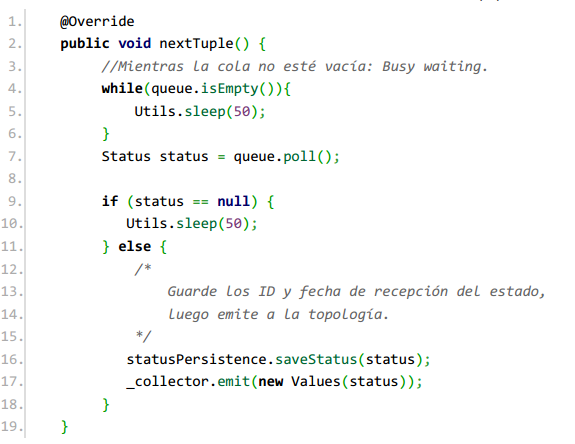
\includegraphics[scale=0.8]{images/TwitterSpout.png}
	\caption[Implementación del \textit{Spout} del sistema.]{Implementación del \textit{Spout} del sistema.}
	\label{fig:TwitterSpout}
\end{figure}

Considerando lo recién expuesto la figura \ref{fig:TwitterSpout} muestra cómo los estados son emitidos por el \textit{spout} al sistema basándose en la cola (\textit{queue}) para manejar lo que llega desde el \textit{stream}.

\subsection{Historia de usuario HU-c02}
\label{subsec:HU-c02}

Esta historia de usuario guarda relación con la HU-v05, menciona la necesidad de incrementar los términos de búsqueda para enriquecerla y abarcar la mayor información posible dado una consulta. Para realizar esto se consideró una práctica del procesamiento de lenguaje natural como es la denominada \textit{Query Expansion} (QE). Según lo descrito por \cite{IRQE} son técnicas comunes al utilizar QE la búsqueda de sinónimos (uso de diccionarios priviamente establecidos), diccionarios basados en la minería de los elementos previamente hayados, creación de diccionadios basados en la co-ocurrencia de términos, es decir, términos que suelen venir juntos o un vocabulario mantenido por editores humanos. Para este trabajo sólo se considerarán las dos primeras: Búsqueda por diccionario de sinónimos y una implementación que encuentra los términos más frecuentes dentro de los resultados de la búsqueda.\\

El diccionario de sinónimos es básicamente una bolsa de palabras asociadas a una semilla, es decir, dado un término de búsqueda agregar todos los términos asociados a el en el diccionario.\\

En el caso de la búsqueda de términos frecuentes se sugirió integrar un proyecto \textit{storm} ya desarrollado el cuál tiene por finalidad la búsqueda de los denominados \textit{thrending topics}, es decir, aquellos términos de los que se realizan más menciones en un determinado instante, pero aquella implementación sólo consideraba los denominados \textit{hashtag}, un marcador de palabras concatenadas que inician por el caracter "\#". Siendo ese el caso el uso de esta topología storm no sería del todo util. En su lugar se desarrolló un contador de frecuencias para palabras con un funcionamiento similar, dicha implementación se aprecia en el algoritmo \ref{alg:TT}.\\

\begin{algorithm}[H]\setstretch{1.5}
	\begin{algorithmic}[numeracion_lineas]
		\REQUIRE Estados $E=\{e_{1}, \dots, e_{n} \}$.
		\ENSURE Terminos frecuentados $T=\{t_{1}, \dots, t_{10} \}$.
		\STATE Lista de terminos: $l$.
		\FOR{Estado: $e_{i}$}
			\STATE Dividir estado por palabra.
			\STATE Eliminar \textit{stopword} de las palabras.
			\FOR{Palabra: $w_{i}$ en $e_{i}$}
				\IF{ $w_{i}$ está en  $l_{i}$}
					\STATE aumentar contador de $w_{i}$ en $l_{i}$.
				\ELSE
					\STATE agregar $w_{i}$ a $l_{i}$ con contador en 1.
				\ENDIF		
			\ENDFOR
		\ENDFOR
		\IF{$l_{i}$ tiene menos de 10 elementos}
			\RETURN $l_{i}$
		\ELSE
			\RETURN los 10 primeros elementos de $l_{i}$.
		\ENDIF
	\end{algorithmic}
	\caption{Algoritmos de términos recurrentes.}
	\label{alg:TT}
\end{algorithm}\vphantom\\

Dado que el operador puede estar replicado no llegarán los mismos estados a todas las instancias del nodo, por ello este proceso se realizará de manera única para cada instancia en función de los estados que hayan llegado a él. El algoritmo \ref{alg:TT} agregará a los términos de búsqueda de cada instancia las palabras más frecuentes y, siguiendo el ejemplo de \textit{Twitter} con sus \textit{thrending topics} tendrá un máximo de diez nuevas palabras.

\subsection{Historia de usuario HU-v00}
\label{subsec:HU-v00}

Dado que una topología de Apache Storm debe ser ejecutada de una forma particular y puede funcionar tanto en un cluster determinado como localmente el integrar la detección de necesidades con un \textit{framework} para construir la interfaz complica el desarrollo. Por ello se decidió separar la visualización y la detección en dos aplicaciones separadas que trabajasen juntas.\\

Teniendo en consideración la característica del desarrollo de esta aplicación como un proyecto ágil con un mínimo de personal para desarrollar se requería de un \textit{framework} que contribuyera a acelerar la construcción de la aplicación. Tras considerar las alternativas más conocidas como \textit{Spring}, \textit{Hibernate} o \textit{JSF} que tienen una curva de aprendizaje elevada, se optó por utilizar un cuarto \textit{framework} que aunque desconocido, prometía una simplicidad en su uso. \textit{Play Framework}, construido haciendo uso de Scala y Java permite construir aplicaciones ligeras (tamaño en disco), sin estado (no guarda configuraciones de una sesión para ser utilizadas luego) y por defecto RESTful, ideal para la comunicación entre aplicaciones. Éste \textit{framework} sigue el patrón de arquitectura Modelo-vista-controlador (MVC). Cuenta con un compilador en tiempo real (compila y realiza el despliegue de la aplicación cuando detecta un cambio en el código), lo que agiliza en gran medida el desarrollo, pues al automatizar este proceso mantiene la atención en lo que se está desarrollando.\\

Para visualizar los puntos encontrados por el detector de necesidades se decidió utilizar la API de \textit{Google Maps} la que permite la colocación de los denominados 'marcadores' en un punto específico del mapa y asociar a ellos algún tipo de información. Así, aunque el funcionamiento interno estará dirigido por \textit{Play}, pero la principal funcionalidad del sistema, mostrar el mapa con sus marcadores, será implementada utilizando Javascript.

\subsection{Historia de usuario HU-v01}
\label{subsec:HU-v01}

Tal como se menciono con respecto a la historia de usuario anterior con el uso de \textit{Google Maps}, ésta historia se completará haciendo uso de los marcadores provistos por esta API. Estos marcadores tendrán asociado un cuadro de texto donde se especificarán los siguientes campos:

\begin{itemize}
\item Contenido del \textit{tweet} que lo generó.
\item Categoría asignada por el sistema
\end{itemize}

De esta manera y dado que la técnica de etiquetado que se utilizó no es del todo precisa permitirá al usuario final discriminar si se ha llegado a un resultado es del todo correcto. El cómo se realizará la categorización de eventos, necesidades en este caso, será detallado en la secciones \ref{subsubsec:7op} y \ref{subsec:clasificacion}.

\subsection{Historia de usuario HU-v02}
\label{subsec:HU-v02}

Desde el punto de vista ingenieríl no presenta mayor desafío, pero sí para fines prácticos. Se prepararon dos tipos de filtro: El primero considera el agrupamiento, mientras que el segundo considera el tipo de marcador.\\

Para el caso del agrupamiento se definieron tres modos de funcionamiento las cuales se describen a continuación:

\begin{enumerate}
\item No agrupar: Muestra todos los marcadores que correspondan en el mapa de acuerdo al punto geográfico que corresponda en su definición.
\item Agrupar por distancia: Define una grilla invisible en el mapa donde los elementos que calcen en una cudrícula son agregados a un \textit{cluster} y visualizados como tal.
\item Agrupar por categoría: Funciona de igual manera que el agrupamiento por distancia, pero sólo agrega elementos que comparan categoría.
\end{enumerate}

Para el segundo caso sólo se definieron dos reglas de funcionamiento las cuales se describen a continuación:

\begin{enumerate}
\item Mostrar todos: Muestra elementos de todas las categorias existentes.
\item Mostrar categoría: Para cada categoría mostrar sólo los elementos de aquella categoría. 
\end{enumerate}

Al combinar ambos tipos de filtros se tienen potencialmente seis modos de funcionamiento, pero considerando las categorías descritas en al sección \ref{subsec:categorias} ese número se expande a veintiún modos de funcionamiento del visualizador.\\

Para implementar esta funcionalidad se utilizan $n + 1$ \textit{clusters}, donde $n$ corresponde al al número de categorías y el cluster extra es para agruparlos a todos. Así si la elección es no agrupar, se muestran todos los marcadores, si la opción es agrupar se insertan todos los marcadores a su respectivo cluster y son mostrados en el mapa y en el caso de querer agrupar, o no, y mostrar sólo una categoría, sólo los elementos, agrupados o no, correspondientes a aquella categoría se ubicarán en el mapa.
 
\subsection{Historia de usuario HU-v03}
\label{subsec:HU-v03}

Se solicitó que la interfaz no se recargue cada vez que se produzca un cambio dado por un nuevo evento detectado o el modificación en el intervalo de visualización. Para ello se utilizaron las facultados de Javascript y AJAX capturando los cambios en la línea temporal, descrita en la sección \ref{subsec:HU-v04}. Cada vez que se detecte un cambio, se eliminará todo marcador del mapa y se reubicarán en el todos los que cumplan con los parámetros de búsqueda.

\subsection{Historia de usuario HU-v04}
\label{subsec:HU-v04}

Al hacer referencia a información pasada se infiere la necesidad de la implementación de un sistema de persistencia de datos.\\

Para ello se consideraron los principales sistemas de bases de datos utilizados y conocidos por el autor, dentro de los cuales se encontraban herramientas como: MySQL, PostgreSQL, SQL Server, MongoDB, entre otras. Dadas las características y las condiciones con las cuales operará el sistema de detección se requiere de un DBMS con rápido tiempo de respuesta en operaciones lectura/escritura; la desición se tomó en base a los datos que se manejaran, pues no se apreció necesidad de implementar una base de datos relacional, de esta forma y teniendo en cuenta los resultados presentados en pruebas empíricas realizadas por \cite{MongoPerformance} en las cuales mostró que el tiempo de respuesta (en operaciones de lectura) es significativamente menor en MongoDB que en dos de los DBMS más conocidos como MySQL y PostgreSQL. Lo anterior, sumado al hecho de la capacidad de escalar de MongoDB reportada en fuentes oficiales o por diversos desarrolladores como \cite{MongoDBScalability} que han compartido sus experiencias en la \textit{web}, llevaron a decidir que MongoDB debiera ser el sistema de gestión de base de datos que se utilizase en el sistema.\\

Para realizar la conexión de MongoDB y \textit{Play framework} se utilizarán, específicamente, dos bibliotecas: La primera corresponde a un ORM (Mapeo Objeto-Relacional), denominado Jongo, la cual hace uso de la segunda llamada Jackson, para realizar la conversion de JSON a objeto.\\

Volviendo al punto; la necesidad de visualizar eventos pasados que involucró la participación de un sistema para persistir los datos, habiendo resuelto lo anterior la siguiente problemática se presenta como ¿qué datos han de guardarse? Según la definición de la historia en la que se señalan "eventos pasados dentro de un intervalo de tiempo", se infiera que ha de guardarse tanto el contenido visible del dato, la clasificación que se le asignó y la fecha en que se identificó, para ello y dado que se seleccionó MongoDB, y aunque no es necesario, se especificó un esquema para los documentos de la colección, dados los datos que se almacenarán sólo restaría tener la información correspondiente a la ubicación, por lo que el esquema se definió como se presenta en la Figura ~\nameref{fig:esquemaMarker1} correspondiente a la colección "Markers".

\begin{figure}[H]
	\centering
	\captionsetup{justification=centering}
	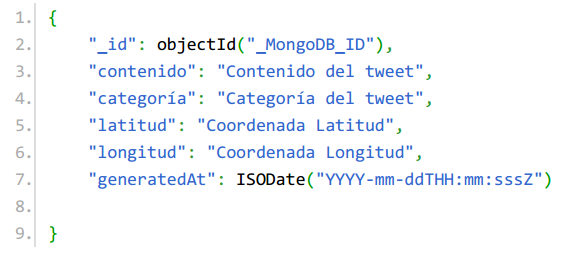
\includegraphics[scale=0.8]{images/Marker1.png}
	\caption[Ejemplo de documento en la colección Markers.]{Ejemplo de documento en la colección Markers.}
	\label{fig:esquemaMarker1}
\end{figure}

Para realizar la selección del intervalo se solicitó, por parte del cliente, el uso de una línea de tiempo con intervalo deslizante que, además, mostrase la cantidad de eventos detectados por fecha por medio de un histograma. Para ello se utilizó, inicialmente, se utilizó \textit{JDateRangeSlider}, de la biblioteca Javascript JQRangeSlider, \cite{JQRangeSlider}. Ésta biblioteca era suficiente para seleccionar el intervalo de fechas y detectar cambios producidos en la línea de tiempo para actualizar los valores, mas no permitía la implementación de un histograma externo.

\begin{figure}[H]
	\centering
	\captionsetup{justification=centering}
	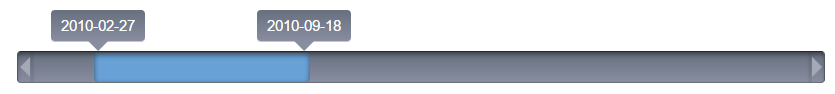
\includegraphics[scale=0.6]{images/JDateRangeSlider.png}
	\caption[Selectorde fechas JDateRangeSlider.]{Selectorde fechas JDateRangeSlider.}
	\label{fig:JQRangeSlider}
\end{figure}

Para lograr implementar ambas dos se utilizó una biblioteca Javascript distinta. La figura \ref{fig:HistogramaFinal} presenta la implementación utilizando \textit{HighCharts}, \cite{Highcharts}. Ésta, al contrario de la anterior, no permitía capturar los cambios en el histograma, para solucionarlo se implementó una función javascript que recogiese los valores del intervalo y arrojara un evento cuando se produjece un cambio, este evento se asoció al eje x de la linea temporal, cambiando el valor de la variable \textit{valuesOfAxis} cada vez que se moviese el eje, éste evento es descrito en la figura \ref{fig:implementacionCambiosEnEje}.\\

Inicialmente este histograma sólo está disponible en inglés, pero permite cambiar todas sus etiquetas manualmente, así, buscando la usabilidad de la aplicación, se modificaron todos los textos y el resultado está visible en la figura \ref{fig:HistogramaFinal}.

\begin{figure}[H]
	\centering
	\captionsetup{justification=centering}
	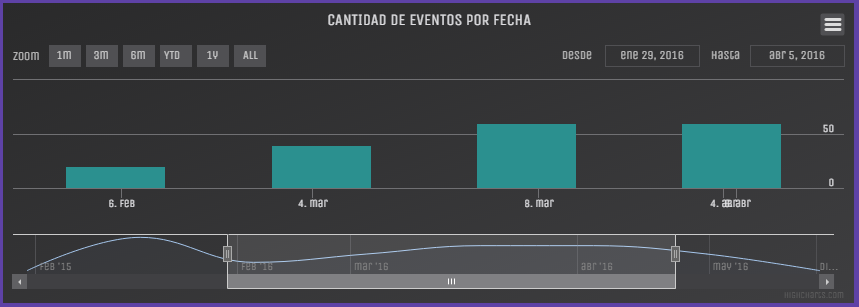
\includegraphics[scale=0.6]{images/Histograma.png}
	\caption[Selector de fechas presente en la aplicación.]{Selector de fechas presente en la aplicación.}
	\label{fig:HistogramaFinal}
\end{figure}

\begin{figure}[H]
	\centering
	\captionsetup{justification=centering}
	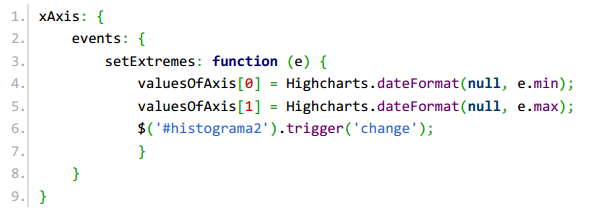
\includegraphics[scale=0.8]{images/onChangeEventTimeline.png}
	\caption[Implementación de evento de detección de cambios en la línea temporal.]{Implementación de evento de detección de cambios en la línea temporal.}
	\label{fig:implementacionCambiosEnEje}
\end{figure}

Tras la selección de intervalo dentro del cual se desea que el sistema muestre los estados recibidos, se implementó un servicio REST, donde mediante una consulta del tipo POST con parámetros fecha inicial y final, retornase una lista con todos los marcadores encontrados.

\subsection{Historia de usuario HU-v05}
\label{subsec:HU-v05}

\textit{Twitter4J}, la herremienta que se mencionó en la sección \ref{subsec:HU-v01} como aquella que permitiría obtener el flujo de información desde \textit{Twitter} implementa una forma de filtrado mediante el uso de palabras clave, pero posee una limitante al momento de modificar la búsqueda, deben instanciarse nuevamente los objetos con los cuales se realiza la conexión a la API de \textit{Twitter}, eso se traduce en tiempo de procesamiento perdido, para solucionar este inconveniente se decidió implementar un operador, descrito en la sección \ref{subsec:operadores}, el cual estará encargado de realizar el filtrado de acuerdo a términos y llevar a cabo la operación descrita en la sección \ref{subsec:HU-c02} referente a la expansión de la consulta, pero siendo un operador significa que sea paralelizado y no exista una sola instancia ¿Cómo comunicar el estado de una consulta y que todos los operadores utilicen el mismo filtro?.\\

Nuevamente la respuesta consistió en recurrir a la base de datos; almacenar la consulta y asignar un estado para controlar el comportamiento del operador. Así el esquema en la base de datos queda tal y como se presenta en la Figura ~\nameref{fig:esquemaQuery}, documento de la colección "Queries".

\begin{figure}[H]
	\centering
	\captionsetup{justification=centering}
	\includegraphics[scale=0.8]{images/Query.png}
	\caption[Ejemplo de documento en la colección queries.]{Ejemplo de documento en la colección queries.}
	\label{fig:esquemaQuery}
\end{figure}

Donde la propiedad "estado" puede tomar dos valores: "actual" o "antiguo", reflejan si una consulta se está llevando a cabo o no. Estos valores son asignados por la aplicación responsable de la interfaz la responsable de recibir los términos de búsqueda por parte del usuario.

Para implementar este operador se utilizaron dos clases llamadas \textit{CurrentQueryChecker} y \textit{QueryExpander} desarrolladas, la primera, para detectar cuándo y si es que ha cambiado una consulta en la base de datos y la segunda para desarrollar la labor descrita por el algoritmo de expansión descrito en la sección \ref{subsec:HU-c02}.

\subsection{Historia de usuario HU-v06}
\label{subsec:HU-v06}

Las categorías mencionadas a continuación son descritas en la sección \ref{subsec:categorias}. Los iconos correspondientes a las categorías que soporta el programa se definieron mediante la combinación de dos imágenes para cada categoría: un marcador de mapa, similar a los definidos en la API de Google Maps y una que sugiriera al usuario el tipo al cual se refería. Los diseños finales son presentados en las figuras de la \ref{fig:agua} a la \ref{fig:seguridad}.\\

\begin{figure}[!htb]
	\minipage{0.32\textwidth}
	\centering
	\captionsetup{justification=centering}
	
\includegraphics[scale=1]{images/categorias/agua.png}
	\caption[Icono categoría agua.]{Icono categoría agua.}
	\label{fig:agua}
	\endminipage\hfill
	\minipage{0.32\textwidth}
	\centering
	\captionsetup{justification=centering}
	
\includegraphics[scale=1]{images/categorias/alimento.png}
	\caption[Icono categoría alimento.]{Icono categoría alimento.}
	\label{fig:alimento}
	\endminipage\hfill
	\minipage{0.32\textwidth}
	\centering
	\captionsetup{justification=centering}
	
\includegraphics[scale=1]{images/categorias/electricidad.png}
	\caption[Icono categoría electricidad.]{Icono electricidad agua.}
	\label{fig:electricidad}
	\endminipage\hfill
\end{figure}

\begin{figure}[!htb]
	\minipage{0.32\textwidth}
	\centering
	\captionsetup{justification=centering}
	
\includegraphics[scale=1]{images/categorias/comunicacion.png}
	\caption[Icono categoría comunicacion.]{Icono categoría comunicacion.}
	\label{fig:comunicacion}	
	\endminipage\hfill
	\minipage{0.32\textwidth}
	\centering
	\captionsetup{justification=centering}
	
\includegraphics[scale=1]{images/categorias/personas.png}
	\caption[Icono categoría personas.]{Icono categoría personas.}
	\label{fig:personas}
	\endminipage\hfill
	\minipage{0.32\textwidth}
	\centering
	\captionsetup{justification=centering}
	
\includegraphics[scale=1]{images/categorias/seguridad.png}
	\caption[Icono categoría seguridad.]{Icono categoría seguridad.}
	\label{fig:seguridad}
	\endminipage\hfill
\end{figure}

Se consideró apropiado, además, diseñar un icono que representara la densidad de marcadores al momento de realizar el agrupamiento por categorías descrito en la sección \ref{subsec:HU-v02} para ello y siguiendo la combinación de colores utilizada por la biblioteca \textit{MarkerClusterer}, \ref{MarkerClusterer}, donde se muestra un cluster azul cuando es un cluster pequeño; amarillo para uno medio y rojo para uno grande. El tamaño de cada uno de estos es especificado internamente por la biblioteca:

\begin{itemize}
\item Azul: De dos a diez elementos.
\item Amarillo: De once a cien elementos amarillo.
\item Rojo: Desde cien elementos.
\end{itemize}

Se prepararon, entonces, tres iconos adicionales a cada categoría para reemplazar los íconos por defecto de la biblioteca, las que pueden verse en las figuras \ref{fig:aguaS}. a la \ref{fig:seguridadL}.\\

\begin{figure}[H]
	\minipage{0.32\textwidth}
	\centering
	\captionsetup{justification=centering}
	
\includegraphics[scale=1]{images/categorias/aguaS.png}
	\caption[Icono categoría agua para cluster pequeño.]{Icono categoría agua para cluster pequeño.}
	\label{fig:aguaS}
	\endminipage\hfill
	\minipage{0.32\textwidth}
	\centering
	\captionsetup{justification=centering}
	
\includegraphics[scale=1]{images/categorias/aguaM.png}
	\caption[Icono categoría agua para cluster medio.]{Icono categoría agua para cluster medio.}
	\label{fig:aguaM}
	\endminipage\hfill
	\minipage{0.32\textwidth}
	\centering
	\captionsetup{justification=centering}
	
\includegraphics[scale=1]{images/categorias/aguaL.png}
	\caption[Icono categoría agua para cluster grande.]{Icono categoría agua para cluster grande.}
	\label{fig:aguaL}
	\endminipage\hfill
\end{figure}

\begin{figure}[H]
	\minipage{0.32\textwidth}
	\centering
	\captionsetup{justification=centering}
	
\includegraphics[scale=1]{images/categorias/alimentoS.png}
	\caption[Icono categoría alimento para cluster pequeño.]{Icono categoría alimento para cluster pequeño.}
	\label{fig:alimentoS}
	\endminipage\hfill
	\minipage{0.32\textwidth}
	\centering
	\captionsetup{justification=centering}
	
\includegraphics[scale=1]{images/categorias/alimentoM.png}
	\caption[Icono categoría alimento para cluster medio.]{Icono categoría alimento para cluster medio.}
	\label{fig:alimentoM}
	\endminipage\hfill
	\minipage{0.32\textwidth}
	\centering
	\captionsetup{justification=centering}
	
\includegraphics[scale=1]{images/categorias/alimentoL.png}
	\caption[Icono categoría alimento para cluster grande.]{Icono categoría alimento para cluster grande.}
	\label{fig:alimentoL}
	\endminipage\hfill
\end{figure}

\begin{figure}[H]
	\minipage{0.32\textwidth}
	\centering
	\captionsetup{justification=centering}
	
\includegraphics[scale=1]{images/categorias/electricidadS.png}
	\caption[Icono categoría electricidad para cluster pequeño.]{Icono categoría electricidad para cluster pequeño.}
	\label{fig:electricidadS}
	\endminipage\hfill
	\minipage{0.32\textwidth}
	\centering
	\captionsetup{justification=centering}
	
\includegraphics[scale=1]{images/categorias/electricidadM.png}
	\caption[Icono categoría electricidad para cluster medio.]{Icono categoría electricidad para cluster medio.}
	\label{fig:electricidadM}
	\endminipage\hfill
	\minipage{0.32\textwidth}
	\centering
	\captionsetup{justification=centering}
	
\includegraphics[scale=1]{images/categorias/electricidadL.png}
	\caption[Icono categoría electricidad para cluster grande.]{Icono categoría electricidad para cluster grande.}
	\label{fig:electricidadÑ}
	\endminipage\hfill
\end{figure}

\begin{figure}[H]
	\minipage{0.32\textwidth}
	\centering
	\captionsetup{justification=centering}
	
\includegraphics[scale=1]{images/categorias/comunicacionS.png}
	\caption[Icono categoría comunicación para cluster pequeño.]{Icono categoría comunicación para cluster pequeño.}
	\label{fig:comunicacionS}
	\endminipage\hfill
	\minipage{0.32\textwidth}
	\centering
	\captionsetup{justification=centering}
	
\includegraphics[scale=1]{images/categorias/comunicacionM.png}
	\caption[Icono categoría comunicación para cluster medio.]{Icono categoría comunicación para cluster medio.}
	\label{fig:comunicacionM}
	\endminipage\hfill
	\minipage{0.32\textwidth}
	\centering
	\captionsetup{justification=centering}
	
\includegraphics[scale=1]{images/categorias/comunicacionL.png}
	\caption[Icono categoría comunicación para cluster grande.]{Icono categoría comunicación para cluster grande.}
	\label{fig:comunicacionL}
	\endminipage\hfill
\end{figure}

\begin{figure}[H]
	\minipage{0.32\textwidth}
	\centering
	\captionsetup{justification=centering}
	
\includegraphics[scale=1]{images/categorias/personasS.png}
	\caption[Icono categoría personas para cluster pequeño.]{Icono categoría personas para cluster pequeño.}
	\label{fig:personasS}
	\endminipage\hfill
	\minipage{0.32\textwidth}
	\centering
	\captionsetup{justification=centering}
	
\includegraphics[scale=1]{images/categorias/personasM.png}
	\caption[Icono categoría personas para cluster medio.]{Icono categoría personas para cluster medio.}
	\label{fig:personasM}
	\endminipage\hfill
	\minipage{0.32\textwidth}
	\centering
	\captionsetup{justification=centering}
	
\includegraphics[scale=1]{images/categorias/personasL.png}
	\caption[Icono categoría personas para cluster grande.]{Icono categoría personas para cluster grande.}
	\label{fig:personasL}
	\endminipage\hfill
\end{figure}

\begin{figure}[H]
	\minipage{0.32\textwidth}
	\centering
	\captionsetup{justification=centering}
	
\includegraphics[scale=1]{images/categorias/seguridadS.png}
	\caption[Icono categoría seguridad para cluster pequeño.]{Icono categoría seguridad para cluster pequeño.}
	\label{fig:seguridadS}
	\endminipage\hfill
	\minipage{0.32\textwidth}
	\centering
	\captionsetup{justification=centering}
	
\includegraphics[scale=1]{images/categorias/seguridadM.png}
	\caption[Icono categoría seguridad para cluster medio.]{Icono categoría seguridad para cluster medio.}
	\label{fig:seguridadM}
	\endminipage\hfill
	\minipage{0.32\textwidth}
	\centering
	\captionsetup{justification=centering}
	
\includegraphics[scale=1]{images/categorias/seguridadL.png}
	\caption[Icono categoría seguridad para cluster grande.]{Icono categoría seguridad para cluster grande.}
	\label{fig:seguridadL}
	\endminipage\hfill
\end{figure}

\subsection{Historia de usuario HU-v07}
\label{subsec:HU-v07}

Específicamente se solicitaron tres tipos de estadísticasa ser mostradas por consulta, estas se definen a continuación:

\begin{enumerate}
\item Cantidad de eventos detectados, es decir, \textit{tweets} que fueron clasificados.
\item Cantidad de usuarios distintos identificados en aquellos eventos.
\item Cantidad total de \textit{tweets} que han pasado por el sistema desde el inicio de la consulta actual.
\end{enumerate}

Para cumplir lo solicitado hacía falta añadir elementos no considerados en la base de datos; hace falta conocer al usuario y contar los \textit{tweets} ingresados desde \textit{Twitter4J}.\\

Para completar esta historia se realizaron modificaciones al esquema previamente definido en la sección \ref{subsec:HU-v04}, este de por si era suficiente para cumplir con la estadística número uno, pero incapáz de realizar las otras dos. Para la segunda estadística se consideró que bastaba con guardar al usuario junto con la colección de marcadores. De acuerdo a \cite{TwitterAgreement} en su sección F. \textit{Be a Good Partner to Twitter}, se insta a los desarrolladores que almacenen contenido \textit{offline} de \textit{Twitter}, a almacenar sólo el ID del usuario o del \textit{tweet}, por ello y siguiendo estos lineamientos se agregará el campo "userID" al esquema marcadores, pasando a quedar como se aprecia en la figura \ref{fig:esquemaMarker2}.

\begin{figure}[H]
	\centering
	\captionsetup{justification=centering}
	\includegraphics[scale=0.8]{images/Marker2.png}
	\caption[Ejemplo de documento en la colección Markers.]{Ejemplo de documento en la colección Markers.}
	\label{fig:esquemaMarker2}
\end{figure}

Para la tercera estadística la colección de marcadores no sería útil, pues no reflejaría la cantidad de tweets procesados, para ello sería necesario implementar una tercera colección de documentos en la base de datos y almacenarlos antes de la aplicación de cualquier tipo de filtro. Esta colección tendrá el esquema presente en la figura \ref{fig:esquemaTweet}.

\begin{figure}[H]
	\centering
	\captionsetup{justification=centering}
	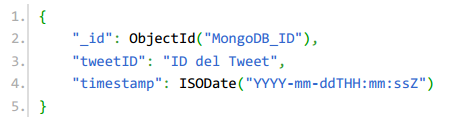
\includegraphics[scale=0.8]{images/status.png}
	\caption[Ejemplo de documento en la colección Status.]{Ejemplo de documento en la colección Status.}
	\label{fig:esquemaTweet}
\end{figure}

Al almacenar sólo el contenido del texto no viola las políticas de uso descritas de \textit{Twitter}, sólo es necesario la fecha para la estadística realizar la estadística, pero resulta útil almacenar el contenido para realizar la expansión de la consulta descrita en la sección \ref{HU-c02} y no aumentar la latencia almacenando el ID y realizando una nueva consulta a la API de \textit{Twitter}.\\

En general la obtención de estas estadísticas se dará utilizando el algoritmo \ref{alg:estadisticas} descrito a continuación.\\

\begin{algorithm}[H]\setstretch{1.5}
	\begin{algorithmic}[numeracion_lineas]
		\REQUIRE Colección $c$ 
		\REQUIRE Fecha de la consulta actual $f$ 
		\ENSURE Contador de eventos $counter$  
		\STATE $counter = 0$
		\FOR{Documento $d_{i}$ en la colección $c$}
			\IF{ fecha de $d_{i}$ es posterior a $f$}
				\STATE $counter = counter + 1$
			\ENDIF	
		\ENDFOR
		\RETURN $counter$
	\end{algorithmic}
	\caption{Algoritmos de generación de primera y tercera estadística.}
	\label{alg:estadisticas}
\end{algorithm}\vphantom\\

Este algoritmo, como se mencionó, es de uso general y permitirá cumplir tanto la primera como la tercera estadística, para el caso de la segunda se requiere una modificación, pues se solicitó conocer los usuarios diferentes, el algoritmo \ref{alg:estadisticas2} presenta el algoritmo modificado para la segunda estadística.\\

\begin{algorithm}[H]\setstretch{1.5}
	\begin{algorithmic}[numeracion_lineas]
		\REQUIRE Colección $c$ 
		\REQUIRE Fecha de la consulta actual $f$ 
		\ENSURE Lista de usuarios vacía $list$  
		\FOR{Documento $d_{i}$ en la colección $c$}
			\IF{ fecha de $d_{i}$ es posterior a $f$}
				\IF{ID del usuario de $d_{i}$ no está en $list$ o $list$ es vacía}
					\STATE Añadir $d_{i}$ a $list$
				\ENDIF
			\ENDIF	
		\ENDFOR
		\RETURN Cantidad de elementos en $list$
	\end{algorithmic}
	\caption{Algoritmos de generación de segunda estadísticas.}
	\label{alg:estadisticas2}
\end{algorithm}\vphantom\\

Adicionalmente a lo anteriormente descrito hace falta un medio para obtener los datos, para ello se implementó un servicio REST donde utilizando un método GET se obtienen todos los datos correspondientes a la actual consulta activa en el sistema, para conocer cuál fue la última consulta del sistema se utiliza la clase \textit{CurrentQueryChecker}, la cual provee de un método para obtener la fecha de la última consulta.

\subsection{Historia de usuario HU-v08}
\label{subsec:HU-v08}

Esta historia nace producto de la HU-v01. El visualizador de eventos tendrá dos maneras de comportarse:

\begin{itemize}
\item Modo tiempo real: Cuando el sistema esté en funcionamiento y cada cierto tiempo, $t_{1}$, se actualizarán los marcadores de los nuevos eventos y éstos se mostrarán durante un tiempo, $t_{2}$.
\item Modo línea de tiempo: Funcionamiento basado en lo descrito en HU-v04.
\end{itemize}

Los tiempos $t_{1}$ y $t_{2}$, inicialmente fueron decididos de manera arbitraria, pero al mostrar su funcionamiento se sugirió que estos parámetros fuesen modificados, por ello, se implementó una sección de configuración dentro de la aplicación de visualización para permitir cambiar estos valores.

\subsection{Operadores}
\label{subsec:operadores}

Como se mencionó en la sección \ref{subsec:HU-c00} la historia de usuario ahí cubierta se encuentra incompleta; Sólo se describió con qué herramienta se apoyará el procesamiento del flujo de información generada al tratarse de un asunto de caracter nacional, pero no se ha definido cómo se capturarán aquellas necesidades.\\

La entrada del sistema se definió en la \ref{subsec:HU-c01} como estados procedentes del flujo de estados desde \textit{Twitter}, pero no se ha hecho mención a la función que tendrá el sistema sobre sobre estos.\\

Tal y como se mencionó en el capítulo \ref{cap:MarcTeorico} una topología \textit{storm} funciona estableciendo un grafo donde cada nodo corresponde a un operador o \textit{bolt}, la figura \ref{fig:stormBeLike} muestra como los \textit{bolt} se unen con el propósito de procesar las entradas entregadas por los \textit{spout} que, en este caso y tal como se señaló en el sección \ref{subsec:HU-c01} corresponderá a aquel que recibe la información desde el \textit{stream} de \textit{Twitter}, pero ¿cuál será la función de cada uno de los \textit{bolts}?\\

La pregunta anteriormente planteada abre un nuevo abanico de problemas, para cada uno de los cuales se desarrollará un operador y éstos, trabajando en conjunto, producirán la información necesaria para ser almacenada como un documento 'marcador' en la colección 'Markers' descrita en la figura \ref{fig:esquemaMarker2}.

\subsubsection{Operador filtro de idioma}
\label{subsubsec:1op}

La primera de las problemáticas a tratar es el idioma. De acuerdo a \cite{TwitterActiveUsers}, existen actualmente 310 millones de usuarios activos en \textit{Twitter} (a enero del 2016), de los cuales 65 millones pertenecen a los Estados Unidos según \cite{TwitterStats1}, y se estima que este año, en latinoamérica, Brasil alcance los 15 millones de usuarios según \cite{TwitterStats2}, sin considerar paises árabes o asiáticos ya se tiene cerca del 30\% de los usuarios activos de \textit{Twitter} hablan, en general, idiomas distintos al Español. Dado que el sistema está pensado para operar dentro de Chile donde el idioma oficial es el Español hace necesario que uno de los operadores, el primero, se el filtrado por idioma, ¿Por qué el primero? Para no realizar procesamiento innecesario con datos que no se utilizarán.\\

\cite{languageDetector} desarrolló, haciendo uso de un clasificador \textit{Naïve Bayes}, un módulo escrito en Java el cual es capaz de detectar con éxito 49 idiomas dentro del texto con un 99.8\% de precisión y fue la primera opción para resolver el problema del idioma, pero al analizar el cuerpo de un estado de \textit{Twitter} se encontró que uno de sus campos, precisamente, correspondía al idioma en el que estaba escrito el \textit{tweet}, por ello, y con objeto de no realizar cálculos innecesarios, se optó por utilizar este campo.\\

La figura \ref{fig:operadorIdioma} presenta el código de la implementación de este \textit{bolt}, correspondiente a su método \textit{execute}, descrito en la sección \ref{subsubsec:Bolt}.

\begin{figure}[H]
	\centering
	\captionsetup{justification=centering}
	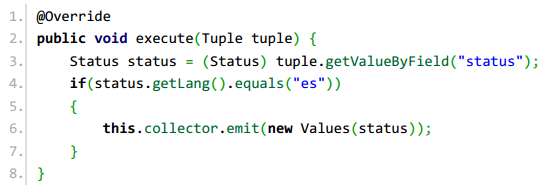
\includegraphics[scale=0.8]{images/LanguageBoltExecute.png}
	\caption[Implementación del método \textit{execute} del \textit{bolt} de idioma.]{Implementación del método \textit{execute} del \textit{bolt} de idioma.}
	\label{fig:operadorIdioma}
\end{figure}

Aunque simple, éste operador filtra un gran número de estados, dado que según lo dicho anteriormente, la mayoría de los usuarios de \textit{Twitter} no son hispano-hablantes. 

\subsubsection{Operador filtro de consultas}
\label{subsubsec:2op}

El segundo problema corresponde a que aunque se tengan los mensajes en el idioma correcto existen mensajes que el usuario desea que sean priorizados, para ello, y como se definió en la sección \ref{subsec:HU-v05}, son entregados términos de búsqueda. Es así como el segundo nivel de operadores corresponderá a aplicar los filtros de búsqueda ingresados por el usuario, si existiesen, aplicando el algoritmo descrito anteriormente y discriminando aquellos estados que contengan las palabras buscadas.

\begin{figure}[H]
	\centering
	\captionsetup{justification=centering}
	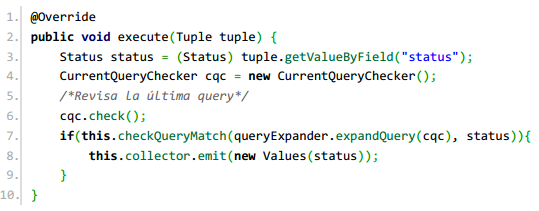
\includegraphics[scale=0.8]{images/FilterBolt.png}
	\caption[Implementación del método \textit{execute} del \textit{bolt} del filtro de consultas.]{Implementación del método \textit{execute} del \textit{bolt} del filtro de consultas.}
	\label{fig:operadorFiltro}
\end{figure}

La figura \ref{fig:operadorFiltro} muestra la implementación del filtro de consultas. Hace uso de instancias de los objetos descritos en HU-v05 para encontrar la última consulta en el sistema y expande la consulta según ésta y los resultados obtenidos en los estados recibidos. Finalmente y si el estado contiene algunos los términos especificados, éste es emitido al siguiente nivel de operadores.

\subsubsection{Operador normalizador de texto}
\label{subsubsec:3op}

El tercer problema es inherente a \textit{Twitter}: En esta red social es común referenciar un estado a un determinado tema, he ahí el uso de los conocidos \textit{Hashtag} que, como se mencionó en la sección \ref{subsec:HU-c02} corresponden a palabras concatenadas antecedidas por el caracter \#. Otro problema común corresponde a la mención de usuarios, ésta corresponde a un llamado al nombre de usuario dentro de la aplicación, antecedida por el caracter "@", usualmente usada para el envío de mensajes entre pares. Diversos autores, entre ellos, \cite{NLPaccuracy}, \cite{NLPaccuracy1} y \cite{NLPaccuracy2}, han señalado que la existencia de estos elementos significan una disminución en la precisión de los elementos descritos en la sección \ref{subsec:clasificacion}. Por ello él tercer operador corresponderá a normalizador de texto, el cual reemplazará menciones a usuarios, \textit{hashtags} y URLs, todas ellas variables, por palabras constantes, el reemplazo a realizarse se muestra en la tabla \ref{tab:reemplazosDeEntidades}. Esto se fundamenta en los resultados descritos en el capítulo \ref{cap:experimentos}.\\

\begin{table}[H]
\centering
\caption{Reemplazo de entidades en texto}
\label{tab:reemplazosDeEntidades}
\begin{tabular}{|c|c|}
\hline
\textbf{Entidad} & \textbf{Reemplazo} \\ \hline
@usuario         & USUARIO            \\ \hline
\#hashtag        & HASHTAG            \\ \hline
http://var.foo/  & URL                \\ \hline
\end{tabular}
\end{table}

La implementación de éste operador se realizo utilizando expresiones regulares para detectar cuándo se está haciendo referencia a uno de los elementos anteriores y luego aplicar su reemplazo.

\subsubsection{Operador geolocalizador}
\label{subsubsec:4op}

El cuarto y mayor problema presentado tiene relación, principalmente, con la historia HU-v01. Si bien se mencionó cómo se realizaría la visualización, no se señaló cómo es que se obtendrían tanto la coordenadas geográficas, latitud y longitud, para ubicar geográficamente un evento.\\

Ha sido señalado por \cite{ChatoSurvey} que menos del 1\% de los \textit{tweets} contienen datos en sus campos correspondientes a geolocalización. En un experimento (véase anexo \ref{anexo:xcentajeGeo}) realizado utilizando la herramienta \textit{RapidMiner} se obtuvo una muestra de 67.789 \textit{tweets} directamente desde el \textit{stream} sin utilizar filtros de búsqueda, de esos \textit{tweets} 67.475 no contaban con los datos correspondientes a la ubicación geográfica, es decir, el 0.46\% de los datos de aquella muestra cuentan con la información requerida, lo que hace creer que lo presentado por los autores, antes mencionados, está en lo correcto.\\

Siendo la geolocalización un elemento de suma importancia para el funcionamiento de la aplicación, se ha de intentar obtener este dato de alguna forma. Así es como surge la posibilidad de usar el contenido del \textit{tweet} para obtener la ubicación, para ello se preparó un diccionario con las comunas del país y sus coordenadas geográficas, \cite{ubicacionesChile} y se diseñó el algoritmo \ref{alg:geolocalizacion}. De esta manera existe una aproximación para detectar la ubicación a la que un \textit{tweet} hace referencia.\\


\begin{algorithm}[H]\setstretch{1.5}
	\begin{algorithmic}[numeracion_lineas]
		\REQUIRE Lista de ciudades $C=\{c_{1}, \dots, c_{n} \}$.
		\REQUIRE Tweet $t$.
		\ENSURE Coordenadas geográficas $P=\{latitud, longitud\}$.
		\IF{$t$ está geolocalizado}
			\IF{Está dentro del territorio chileno}
				\RETURN Coordenadas del $t$.
			\ELSE
				\RETURN Fuera de Chile.
			\ENDIF
		\ELSE
			\IF{El texto de $t$ contiene elementos presentes en $C$}
				\RETURN Coordenadas de $c_{i}$.
			\ELSE
				\RETURN No geolocalizable.
			\ENDIF
		\ENDIF
	\end{algorithmic}
	\caption{Algoritmos de ubicación geoográfica.}
	\label{alg:geolocalizacion}
\end{algorithm}\vphantom\\

Para detectar cuándo una ubicación está en Chile, se generó un cuadro en el mapa donde se delimita todo el territorio Chileno, incluyendo Isla de Pascua.\\

Haciendo uso del algoritmo desarrollado es posible aumentar la cantidad de elementos que continuarán en la línea de procesamiento. En el capítulo \ref{cap:experimentos} realiza una evaluación sobre la efectividad del operador.\\

Los operadores descritos en las secciones \ref{subsubsec:5op} y \ref{subsubsec:6op} tienen relación con la labor del señalado en \ref{subsubsec:7op}, las razones que llevan a la construcción de estos tres serán expuestan en la sección \ref{subsec:clasificacion}, mientras tanto, al igual que los operadores anteriores se detallará el cómo fueron diseñados.

\subsubsection{Operador removedor de \textit{stopword}}
\label{subsubsec:5op}

Éste operador hará uso de una lista de palabras denominadas \textit{stopwords} o palabras vacías, éstas corresponden a palabras sin significado, como artículos, pronombres, preposiciones, etcétera. Éstas palabras serán eliminadas del texto que se está procesando, para ello se utilizará el algoritmo presentado a continuación.\\

\begin{algorithm}[H]\setstretch{1.5}
	\begin{algorithmic}[numeracion_lineas]
		\REQUIRE Lista de \textit{stopwords} $S=\{s_{1}, \dots, s_{n} \}$.
		\REQUIRE Texto $T$.
		\ENSURE Texto $T'$.
		\STATE $T'$ = $T$
		\FOR{cada palabra de $T$, $t_{i}$}
			\IF{$t_{i}$ está contenida en $S$}
			\STATE $T'$ = $T'$ - $t_{i}$. 
			\ENDIF
		\ENDFOR
		\RETURN $T'$
	\end{algorithmic}
	\caption{Algoritmos de eliminiación de \textit{stopwords}.}
	\label{alg:stopwords}
\end{algorithm}\vphantom\\

\subsubsection{Operador raíz de texto}
\label{subsubsec:6op}

Este operador hace uso del algoritmo de \cite{Porter}, para extraer prefijos y sufijos de palabras y llevarlas a una raíz común, \cite{StemmingLema}, son ejemplos de este proceso, denominada \textit{stemming}, las palabras presentadas en la tabla \ref{tab:ejstemming}

\begin{table}[H]
\centering
\caption{Ejemplo de \textit{stemming} para la palabra 'presentar'}
\label{tab:ejstemming}
\begin{tabular}{|c|c|}
\hline
\textbf{Palabra} & \textbf{Combinaciones de Sufijos} \\ \hline
Presentarla      & arla                              \\ \hline
Presentarlas     & arlas                             \\ \hline
Presentarle      & arle                              \\ \hline
Presentarles     & arles                             \\ \hline
Presentarlo      & arlo                              \\ \hline
Presentarlos     & arlos                             \\ \hline
Presentarse      & arse                              \\ \hline
Presentase       & ase                               \\ \hline
Presentásemos    & ásemos                            \\ \hline
Presente         & e                                 \\ \hline
Presentémonos    & émonos                            \\ \hline
\end{tabular}
\end{table}

\subsubsection{Operador etiquetador}
\label{subsubsec:7op}

Este operador hace uso del clasificador generado mediante las técnicas descritas en la sección \ref{subsec:categorias}, para etiquetar el texto de acuerdo a la categoría a la que corresponda. Una vez realizado este proceso se cuenta con todos los datos necesarios para generar completamente un documento de la colección 'Markers', presentada en la figura \ref{fig:esquemaMarker2}.

\subsubsection{Operador persistencia}
\label{subsubsec:8op}

Este operador se encargará de conectarse a la base de datos y almacenar el nuevo marcador. Los datos recibidos desde la cadena de procesamiento se llevarán a una instancia de objeto Java, llamado "Marker", el cual contiene los mismos elementos descritos para un documento de la colección "Markers", a un objeto JSON utilizando \textit{Jackson} y finalmente, utilizando \textit{Jongo}, lo transformará en BSON para almacenarlo en la base de datos en MongoDB.

\subsection{Clasificación}
\label{subsec:clasificacion}

Hasta ahora se han tocado, prácticamente, todos los temas que se relacionan con el funcionamiento del sistema de detección, desde donde se obtendrán los datos, cómo se procesaran e incluso cómo se almacenaran, pero no se ha especificado cómo se realizará la clasificación, es decir, cómo dado un texto de entrada se conseguirá discriminar en qué categoría encaja. Ésta sección especifica lo que se contextualizó en la sección \ref{subsubsec:7op}.\\

El proyecto PMI realizado por \cite{WladdimiroPMI}, como se mencionó en en el capítulo \ref{cap:introduccion}, abordó una solución inicial para el problema de la detección de necesidades. En aquella oportunidad se utilizó una bolsa de palabras con términos asociados a las categorías para etiquetar los estados de \textit{Twitter}. Este trabajo busca mejorar aquello realizando la clasificación mediante una técnica de clasificación más poderosa.\\

En su libro, \textit{Introduction to Information Retrival}, \cite{IRQE}, proponen el uso de \textit{Naïve Bayes}, para realizar clasificación de texto. Esto se logra realizando una implementación del algoritmo descrito en la sección \ref{subsec:naiveBayes}. Este ya ha sido implementado en diversas herramientas como: RapidMiner, Weka (acrónimo de \textit{Waikato Envoirment for Knowledge Analysis}), Mallet (acrónimo de \textit{MAchine Learning for LanguagE Toolkit }).\\ 

Tras haber realizado pruebas con ellas se decidió utilizar Mallet por su simplicidad de implementación junto con la mayor precisión de sus resultados.\\

El concepto que involucra la construcción de un clasificador es el de "aprendizaje supervizado", que fue mencionado en la sección \ref{sec:aprendSuperv}, en este tipo de aprendizaje se requiere de un conjunto de datos de entrada, denominados conjunto de entrenamiento, que ha de pasar por el algormito, en este caso \textit{Naïve Bayes}, que ha de conocer previamente, la salida esperada para cada elemento del conjunto. El resultado esperado es un clasificador capáz de predecir, en este caso, a qué categoría pertenece un texto sometido a su evaluación.\\

Según la metodología KDD existen cinco pasos en la búsqueda de conocimiento en bases de datos, estos fueron descritos en la sección \ref{subsec:kdd}, pero son enunciados aquí para ilustrar en qué punto se está del proceso general:

\begin{enumerate}
\item Selección.
\item Preprocesamiento.
\item Transformación.
\item Minería.
\item Evaluación.
\end{enumerate}

La selección de datos se ha llevado a cabo. Se cuenta con más de 2000 estados recogidos desde \textit{Twitter} previo, durante y posterior al terremoto de Concepción el año 2010. Éstos datos se han etiquetado por el autor, dándoles la categoría a la que hacen referencia.\\

El siguiente paso a realizarse según la metodología es realizar un preprocesamiento. Según lo descrito por \cite{IRQE}, se sugiere emplear una serie de técnicas tanto para preprocesar como transformar los datos, éstas son:

\begin{itemize}
\item Tokenización: Dada una secuencia de carácteres y una unidad definida (una palabra en este caso), la tarea es cortar esa secuencia en \textit{Tokens} y, a la vez, eliminar ciertos carácteres (por ejemplo, signos de puntuacion).
\item Eliminación de stopwords: Son elementos que no aportan a la selección en el proceso de clasificación, usualmente se mantienen en una lista y son eliminados de la secuencia.
\item Normalización: Incluye los procesos de llevar todo el texto a minúsculas o mayúsculas, llevar términos a equivalencias, seleccionar el idioma, etcétera.
\item \textit{Stemming}: Llevar los términos a una raíz común.
\end{itemize}

Estas transformaciones han sido descritas por los operadores anteriores con excepción de aquellos que tienen que ver con el filtrado de consultas, la ubicación de \textit{tweets}, el etiquetado propiamente tal y la persistencia.\\

Para la construcción del clasificador, cada conjunto de datos pasará obligatoriamente por todos estos procesos.\\

\subsection{Categorías de clasificación}
\label{subsec:categorias}

La definición de las categorías es un punto importante dentro de la construcción de la aplicación. Teóricamente en función a la cantidad de clases (categorías), el tamaño del conjunto de entrenamiento ha de ser mayor o menor.\\

Inicialmente se consideró la taxonomía definida por \cite{TaxonomiaChato}, pero el cliente mencionó que no era conveniente utilizar, pues presentaba gran cantidad de categorías y era demasiado específica, se sugirió en su lugar utilizar la clasificación realizada por \cite{Alvarado} en la que se presentaba una categorización de cinco categorías, ellas eran:

\begin{enumerate}
\item Necesidades básicas: \textit{Tweet} que entregara o solicitara información sobre serviciós básicos: Agua potable, electricidad y abastecimiento de alimentos.
\item Comunicación: \textit{Tweet} que entregue o solicite información sobre alguna localidad.
\item Seguridad: \textit{Tweet} que señale un riesgo para la población.
\item Personas: \textit{Tweet} que haga referencia al hallazgo o búsquead de una persona desaparecida.
\item Irrelevante: Cualquier otro \textit{tweet}.
\end{enumerate}

Acordando con el cliente, se decidió separar el primer ítem en los tres elementos que lo componen: Agua, alimentos y electricidad. Así, finalmente, se obtienen siete categorías de clasificación.\\

Los elementos clasificados como "Irrelevantes" no se mostrarán en el mapa de eventos, pues hacen referencia a eventos que, pese a haber pasado por todos los operadores anteriormente descritos, no guardan relación con el evento o sus consecuencias.


\subsection{Clasificador}
\label{sec:clasificador}

La sección \ref{subsubsec:7op} define la existencia del operador encargado de etiquetar los nuevos estados, no será éste el encargado de la construcción del clasificador, pues al tratarse de un aprendizaje supervisado, requiere de una persona que realice el etiquetado mediante el cual se realiza el entrenamiento.\\

Al no poder automatizar el proceso antes señalado se consultó con el cliente si es que aceptaría la implementación de un actualizador manual del clasificador´, lo cual se aceptó.\\

El actualizador del clasificador realizará los procesos descritos aquí, previos al etiquetado, de manera que para cualquier entrada que cumpla el formato descrito en la figura \ref{fig:formatoFig} permitirá la construcción de un nuevo clasificador.\\

\begin{figure}[H]
	\centering
	\captionsetup{justification=centering}
	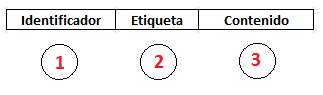
\includegraphics[scale=0.8]{images/FormatoArchivoEntrada.png}
	\caption[Formato archivo de entrada.]{Formato archivo de entrada.}
	\label{fig:formatoFig}
\end{figure}

\begin{enumerate}
\item Corresponderá a un identificador arbitrario, pero necesario para la herramienta de clasificación Mallet.
\item Corresponderá a la etiqueta que categoriza al contenido.
\item Contenido del \textit{tweet} propiamente tal.
\end{enumerate}

Teniendo en consideración que se utilizan dos aplicaciones distintas, donde en una se construirá el clasificador y en otra se utilizará surge el problema de cómo realizar la comunicación entre ellas. Para solucionar este inconveniente se utilizará una carpeta compartida por ambas aplicaciones. En el caso de sistemas Unix se utilizará el directorio $/opt/DeNe$, mientras que para Windows se utilizará $C:/DeNe/$. En estos directorios se almacenará un fichero con el clasificador serializado.

\begin{figure}[H]
	\centering
	\captionsetup{justification=centering}
	
\includegraphics[scale=0.8]{images/ClasifierDene.png}
	\caption[Fichero clasificador en $c:/DeNe/$.]{Fichero clasificador en $C:/DeNe/$.}
	\label{fig:TopologiaGeneral}
\end{figure}

Cada vez que se actualice el clasificador se contrastará el nuevo con el ya existente, de encontrar mayor presición en el primero, se reemplazará. En caso contrario , se mantendrá al anterior. En ambos escenarios se le dará a conocer al usuario la precisión de ambos.

\subsection{Topología del sistema}
\label{subsec:topologiaSistema}

Habiendo definido los elementos de procesamiento, los operadores o \textit{bolts}, se está en condicion de definir la topología. La topología que utilizará el sistema, en términos generales de la aplicación está definida en la figura \ref{fig:TopologiaGeneral}.

La razón de este orden en la topología se debe a varias razones y se justifican a continuación:

\begin{itemize}
\item \textit{Spout Twitter}: Es el eslabón principal de la cadena. Desde aquí se emitirán los nuevos estados al sistema y todo el sistema depende de el. 
\item \textit{Bolt} Filtro de idioma: Ocupa la primera posición de los operadores del sistema, dado que se espera que el \textit{stream} reciba estados de todo el mundo y no sólo en español. Al estar este operador en primer lugar se asegura de reducir el flujo en gran medida.
\item \textit{Bolt} Filtro de consulta: Habiendo filtrado sólo aquellos estados cuyo lenguage sea el español es necesario filtrar aun más el \textit{stream} valiéndose de las restricciones especificadas por el usuario. Así sólo los estados que contengan términos especificados por el usuario, o el sistema de expansión, continuarán en el sistema.
\item\textit{Bolt} Normalizador de texto: Previo al detector de ubicación para evitar posibles confusiones que pueda acarrear la existencia de nombres de lugares en elementos como nombres de usuario, \textit{hashtags} o enlaces.
\item\textit{Bolt} Detección de ubicación: Ocupa esta posición, pues debe ir previo a la eliminación de \textit{stopwords}, de no ser así ubicaciones, como por ejemplo, "los vilos", no serían detectados al realizar la comparativa en éste operador.
\item\textit{Bolt} Eliminador de \textit{stopword}: Se realiza previo al \textit{Stemming} para reducir la carga computacional, pues el operador de \textit{stemming} llevaría a palabras raíz estos términos que no son necesarios.
\item\textit{Bolt} \textit{Stemmer}: Es la única ubicación posible para este operador, pues el siguiente paso es etiquetar el estado.
\item\textit{Bolt} Etiquetador: Aplica el modelo al estado, el estado ha de tener su correspondiente etiqueta antes de ser almacenado.
\item\textit{Bolt} Persistencia: último eslabón de la cadena. Ingresa un nuevo documento a la colección de marcadores.
\end{itemize}

\begin{figure}[H]
	\centering
	\captionsetup{justification=centering}
	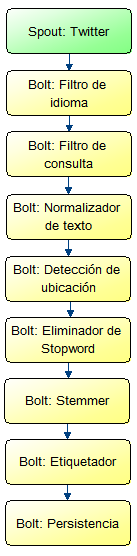
\includegraphics[scale=0.8]{images/TopologiaGeneral.png}
	\caption[Topología general del sistema.]{Topología general del sistema.}
	\label{fig:TopologiaGeneral}
\end{figure}

\subsection{Arquitectura del sistema}
\label{subsec:Arquitectura}

Ya se ha mencionado que el sistema completo constará de dos aplicaciones: el visualizador que, además permitirá actualizar el clasificador, y la aplicación detectora de necesidades. Considerando lo anterior se presenta la arquitectura del sistema en la figura \ref{fig:arquitecturaSistema}. En ella se aprecia que los datos llegan al sistema desde \textit{Twitter} y, utilizando Apache Storm para soportarlo, además del clasificador, son clasificados, detectando necesidades y almacenando, en la base de datos, los nuevos marcadores, luego, en la aplicación visualizadora, haciendo uso de Google Maps, son mostrados en el cliente \textit{web} por medio de su navegador.

\begin{figure}[H]
	\centering
	\captionsetup{justification=centering}
	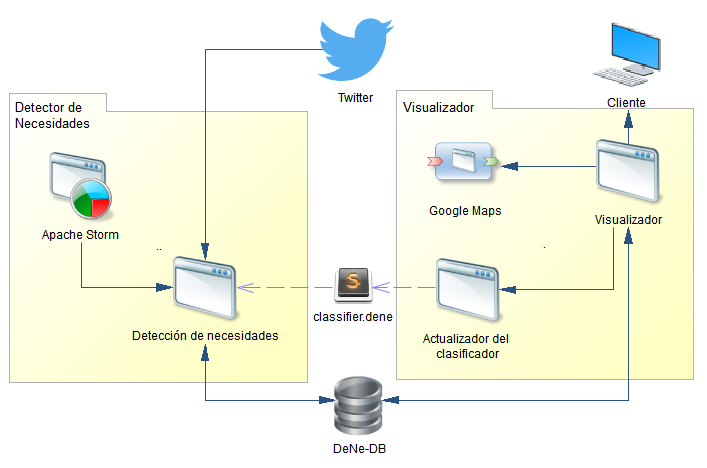
\includegraphics[scale=0.8]{images/arquitecturaGeneral.png}
	\caption[Arquitectura del sistema.]{Arquitectura del sistema.}
	\label{fig:arquitecturaSistema}
\end{figure}

\subsection{Funcionamiento y comportamiento}
\label{subsec:FuncionamientoYComportamiento}

El sistema descrito está diseñado para operar de forma continua en condiciones de alto tráfico como lo es al ocurrir una emergencia del tipo catastrófica en el país.\\

Se asumirá que existe un sistema externo que estará encargado de detectar cuándo se produzca una situacion de las características antes mencionadas y comience a ejecutar el sistema de detección, pues no está dentro de los alcances de este trabajo el que se detecte  cuándo es que se ha producido un evento y la población comience a producir nuevos estados en las redes sociales.
